\chapter{複素函数}%第2章

\begin{mysimplebox}{問1}
    点集合$E\subset\C$が閉集合であるためには$E$の境界$\partial E$が$E$の部分であることが必要十分であることを示せ。 
\end{mysimplebox}

本の定義では$E$が閉であるとは$E$の集積点がすべて$E$に属することである(p.22)。点$c$が$E$の集積点であるとは、任意の正数$r$に対して、$0<|z-c|<r$を満たすような$E$の点$z$が存在することである(p.21)。この集積点の定義では、$|z-c|=0$となる$z$は除いていることに注意が必要である。すなわち$c\in E$である必要はないということである。

\paragraph{証明}
($\Rightarrow$)
$E$は閉であるとしたとき、$\partial E\subset E$であることを示す。
すなわち、$x\in\partial E$ならば$x\in E$であることを示す。
$r\in\R$に対して
\begin{align*}
    B_r(x)=\left\{y\in\C\mid|y-x|<r\right\}
\end{align*}
と定義する。$E$の境界$\partial E$の点$x$は$E$の内点でも外点でもない。特に、外点でないことから、任意の$n\in \N$に対して、$B_{1/n}(x)$は$E$と交わりをもつ。よって、任意の$n\in \N$に対して、$x_n\in B_{1/n}(x)\cap E$をとれる。

もし$|x-x_n|=0$となる$n\in\N$が存在すれば、$x=x_n\in E$である。

すべての$n\in\N$に対して$|x-x_n|\neq 0$であるとする。$|x-x_n|\longrightarrow 0\, (n\longrightarrow \infty)$であり、$\{x_n\}\subset E$であるから、$x$は$E$の集積点である。したがって、$E$は閉であると仮定していたから、閉であることの定義より$x\in E$である。

(集合の集積点は、その集合に属している必要はないという、集積点の定義に応じて場合分けを行った)

\begin{figure}
    \centering
    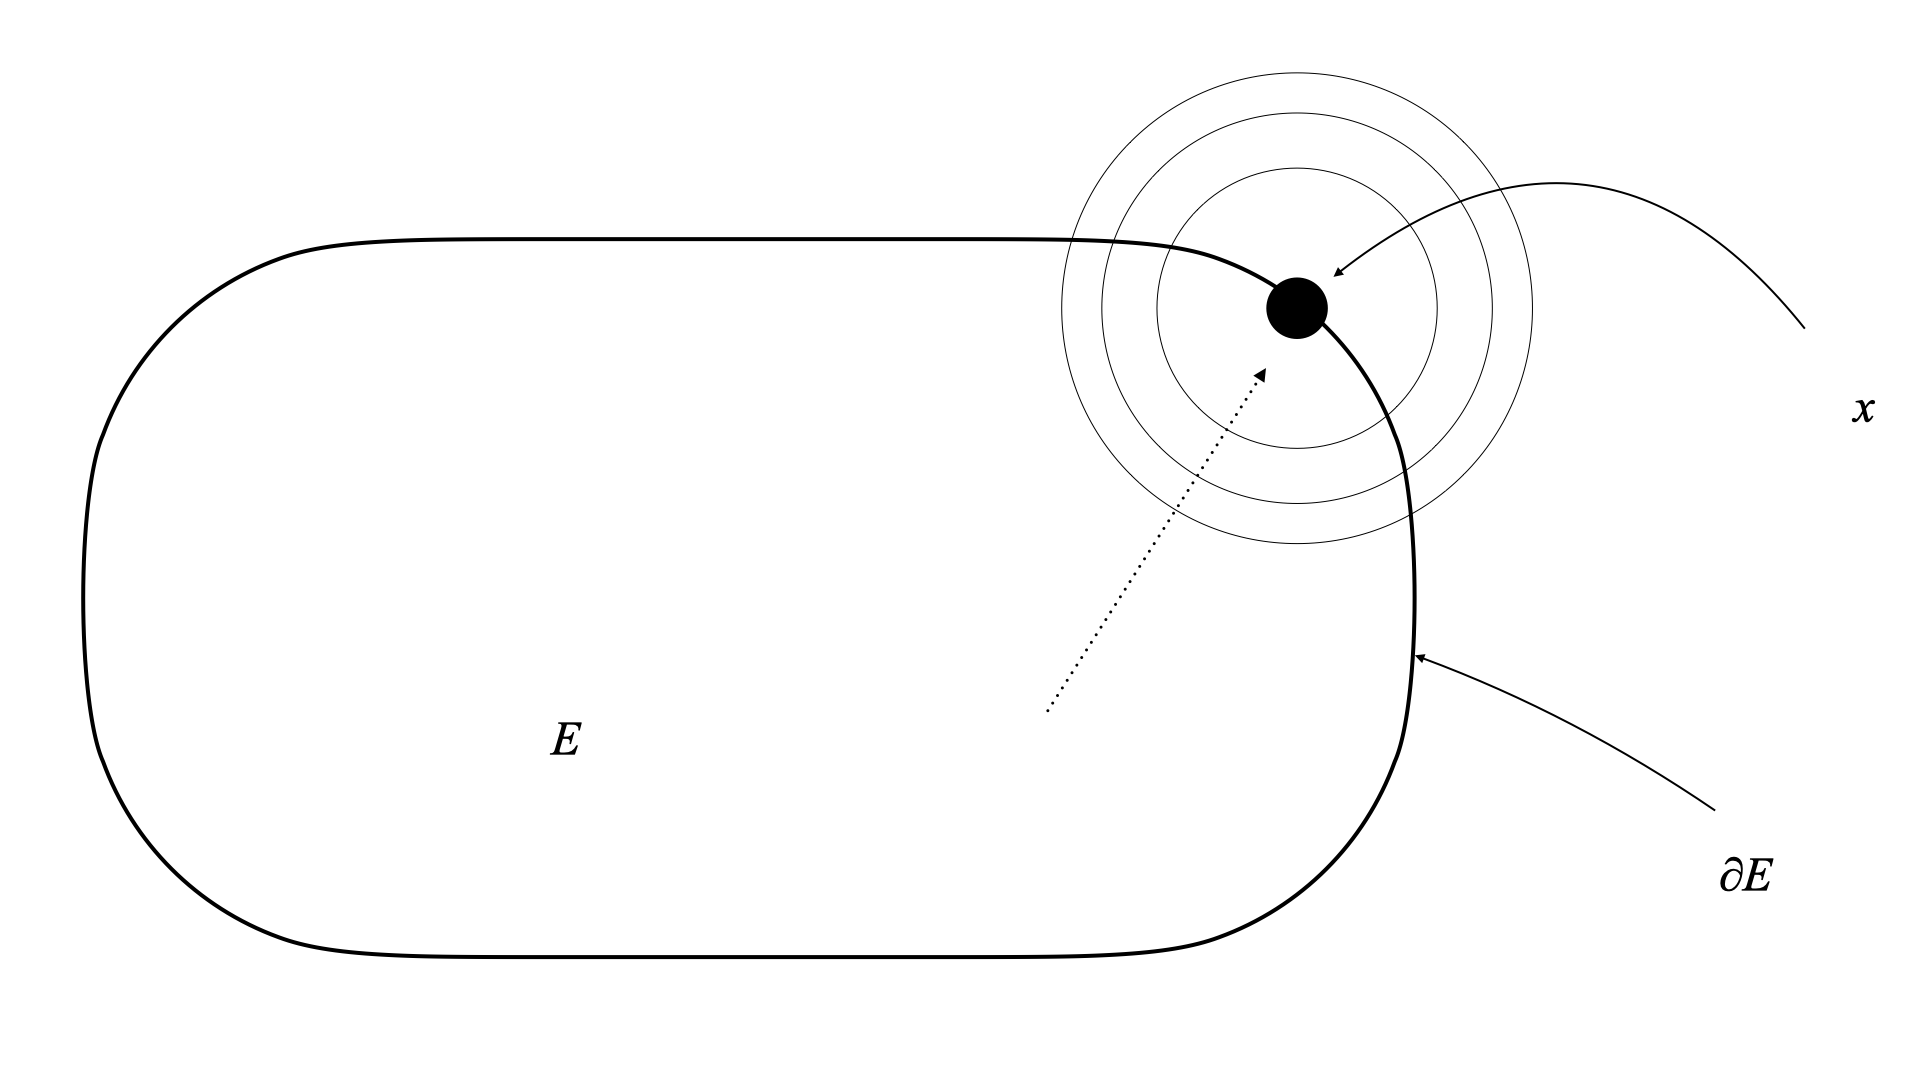
\includegraphics[width=6cm]{ch2_prob1_1.png}
    \caption{閉集合$E$と境界$\partial E$}
    \label{ch2_prob1_1}
\end{figure}%

($\Leftarrow$)
$\partial E\subset E$とする。$x$が$E$の任意の集積点であるとき、$x\in E$であることを示せばよい($E$が集積点をもたないとき$E$は孤立点のみからなるが、そういった集合は閉であると定義し直しておく)。ここで、$\C$の任意の点は$E$の内点か外点か境界の点であることに注意する。

もし$E$の集積点$x$が$E$の外点であるとすると、ある$r\in\R$に対して$B_r(x)\subset E^c$($E^c$は$E$の補集合を表す)であるから、$x$が$E$の集積点であることに反する。

よって、$E$の集積点$x$は$E$の内点か境界の点である。内点ならば$x\in E$は明らかである。境界の点ならば$\partial E\subset E$という仮定から、やはり$x\in E$である。(証明終)

\begin{mysimplebox}{問2}
    点集合の境界は閉集合であることを示せ。 
\end{mysimplebox}
\paragraph{証明}
$E$を点集合とし、$x$を$\partial E$の集積点とする。$x\in\partial E$であることを示せばよい。

$x$を$E$の内点とすると、ある$n\in\N$に対して、$B_{1/n}(x)\subset E$である。一方、$x$は$\partial E$の集積点であるから、ある$y\in\partial E$が存在して、$y\in B_{1/n}(x)\subset E$である。十分小さい$n'\in\N$をとれば、$B_{1/n'}(y)\subset E$であるから、$y$は$E$の内点である。しかし、これは$y\in\partial E$に反する。よって$x$は$E$の内点ではない。

$x$を$E$の外点としても同様の議論ができるから、$x$は$E$の外点でもない。

したがって、$x$は$E$の境界の点である。(証明終)

\begin{mysimplebox}{問3(Borel--Lebesgueの被覆定理)}
    有界な閉集合$E\subset\C$の各点においてそれぞれ1つの近傍が与えられているとする。
    そのとき、これら無数の近傍の中から有限個を選び出して、
    $E$のいかなる点もこれら有限個の近傍のいずれかに含まれるようにできる。
    これを示せ。
\end{mysimplebox}
\paragraph{証明}
有界な閉集合$E$の各点においてそれぞれ1つの近傍が与えられているとする。
このとき、$E$が有限被覆可能でないと仮定して矛盾を導く。

$E$が4点$R+Ri, -R+Ri, -R-Ri, R-Ri$を頂点とする閉正方形$Q_0$
に包まれるように正数$R$を大きくとる。$E$が有界であることから、これは可能である。

$Q_0$の対辺の中点を結んで$Q_0$を4つの閉正方形に分けると、
そのうちの少なくとも1つと$E$との共通部分は有限被覆可能でない。
その閉正方形を$Q_1$とする。

この手続きを繰り返して、閉正方形の列
$Q_0, Q_1, Q_2,\dots$を作る。
各$Q_k$と$E$の共通部分は、最初に与えられた$E$の各点の近傍に関して、
有限被覆可能ではない。

$Q_k\cap E$は空ではないから、各々の$k$に対して$q_k\in Q_k\cap E$となる点列$\{q_k\}$をとることができる。$\{q_k\}$は有界である。よって、Weierstrass--Bolzanoの定理により、$\{q_k\}$の部分列の中に
収束するものが存在する。
%例えば閉正方形$Q_k$の右上の頂点を$a_k+b_{k}i (a_k,b_k\in\R)$、
%左下の頂点を$c_k+d_{k}i (c_k,d_k\in\R)$とすると、
%$\{a_k\}, \{b_k\},\{c_k\},\{d_k\}$にも収束する部分列がある。
%$a_k-c_k=b_k-d_k=\frac{2R}{2^k}$であり、$k\longrightarrow\infty$の極限で0に収束するため、
%区間縮小法により、$\{Q_k\}$の収束する部分列は1点に収束する。
$\{q_k\}$の収束するある部分列を$\{q_{k_l}\}$とし、その収束点を$q$とする。

$\{q_{k_l}\}$の各項は$Q_{k_l}\cap E$の点であるから、
$q$は$E$の集積点である。
$E$が閉であることから$q\in E$である。

したがって、最初に$E$の各点に与えられた近傍として、
$q$にも近傍$V_q$が与えられており、
十分大きい$l$ に対して$Q_{k_l}\subset V_q$である。

これは$Q_{k_l}$が有限被覆可能でないことに反する。(証明終)

\begin{mysimplebox}{問4}
    $c$が定数のとき$|z-c|$は全平面で連続な函数であることを示せ。
\end{mysimplebox}
\paragraph{証明}
$f(z)=|z-c|$とする。
\begin{align*}
    f(z)-f(z')&=|z-c|-|z'-c|\\
    &\le |(z-c)-(z'-c)|\\
    &=|z-z'|
\end{align*}
よって、任意の$z\in\C$、任意の$\epsilon>0$に対して
$|z-z'|<\epsilon$となるように$z'\in\C$をとれば
$|f(z)-f(z')|<\epsilon$とできる。
ゆえに$f(z)$は全平面で連続である。(証明終)

\paragraph{補足}
この証明によって$f(z)$は一様連続であることが示された。

\begin{mysimplebox}{問5}
    点$c$と閉集合$E$の距離が$d$ならば$d=|z-c|, z\in E$となる$z$が存在することを示せ。
\end{mysimplebox}
\paragraph{証明}
\begin{align*}
    d\coloneqq \inf_{z\in E}|z-c|
\end{align*}
である。

$d=|z-c|$となる$z\in E$が存在しないと仮定すると、
下限の定義により、任意の正の整数$n$に対して$d<|z_n-c|<d+\frac{1}{n}$となる$z_n\in E$をとることができる。

点列$\{z_n\}$は有界な無限列であるから、
収束する部分列$\{z_{n_k}\}$を有する。
$z_{n_k}\longrightarrow c'$とする。$c'$は$E$の集積点であり、$E$は閉集合であるから$c'\in E$である。

仮定より$|c'-c|>d$であるから$|c'-c|>|z_{n_k}-c|>d$となる$z_{n_k}\in E$が存在する。しかし$z_{n_k}\longrightarrow c'$であり、
\begin{align*}
    |z_{n_k}-c|>|z_{n_{k+1}}-c|>\dots>|c'-c|.
\end{align*}
よって矛盾である。(証明終)

\paragraph{補足}
収束する部分列の収束点$c'$に対して、$c'\in E$であるから$d\le|c'-c|$は明らかである。一方、
\begin{align*}
    |c'-c|\le|c'-z_{n_k}|+|z_{n_k}-c|< \epsilon + d+\frac{1}{n_k}
\end{align*}
である。$\epsilon+\frac{1}{n_k}$はいくらでも小さくできるから、$|c'-c|\le d$である。

よって、$d=|c'-c|$である。

\begin{mysimplebox}{問6}
    $E, E'$がともに閉集合で、そのうちの1つが有界であるとき、$E$と$E'$の距離が$d$ならば$d=|z-z'|, z\in E, z'\in E'$となる$z, z'$が存在することを示せ。
\end{mysimplebox}
\paragraph{証明}
\begin{align*}
    d\coloneqq \inf_{z\in E, z'\in E'}|z-z'|
\end{align*}
である。

$E\cap E'\neq \emptyset$ならば、$d=0$であり、$z\in E\cap E'$
に対して$|z-z|=0=d$となり証明が終わる。

$E\cap E'=\emptyset$とする。$E$と$E'$の距離が$d$であるとする。
また、$E$は有界であるとする。
$d=|z-z'|$となる$z\in E, z'\in E'$が存在しないとすると、
\begin{align*}
    |z_1-z'_1|>|z_2-z'_2|>\dots>d
\end{align*}
となる列$\{z_k\}_{k=1,2,\dots}\subset E, \{z'_k\}_{k=1,2,\dots}\subset E'$が存在する。

$E$は有界であるから、$\{z_k\}$は収束する部分列を有する。
それを$\{z_{k_l}\}_{l=1,2,\dots}$とし、$z_{k_l}\longrightarrow c$とする。$c$は$E$の集積点であり$E$は閉集合であるから、$c\in E$である。

ここで$\{z_{k_l}\}_{l=1,2,\dots}$に対応する$\{z'_{k_l}\}_{l=1,2,\dots}$について考える。
任意の$\epsilon>0$に対して$l$を十分大きくとれば、
$d<|z_{k_l}-z'_{k_l}|<d+\epsilon/2$とできる。
また同時に$|c-z_{k_l}|<\epsilon/2$とできる。
よって$|c-z'_{k_l}|\le|c-z_{k_l}|+|z_{k_l}-z'_{k_l}|<\epsilon/2+d+epsilon/2=d+\epsilon$である。
すなわち$\{z'_{k_l}\}_{l=1,2,\dots}$は有界であるから、収束する部分列を有する。
それを$\{z'_{k_{l_m}}\}_{m=1,2,\dots}$とし、$z'_{k_{l_m}}\rightarrow c'$とする。
$c'$は$E'$の集積点であり$E'$は閉集合であるから、$c'\in E'$である。

仮定より$|c'-c|>d$であるから$|c'-c|>|z_{k_{l_m}}-z'_{k_{l_m}}|>d$となる$m$が存在する。しかし$z_{k_{l_m}}\longrightarrow c$、$z'_{k_{l_m}}\longrightarrow c'$であり、
\begin{align*}
    |z_{k_{l_m}}-z'_{k_{l_m}}|>|c-c'|.
\end{align*}
よって矛盾である。(証明終)

\paragraph{別証}
$E$は有界閉集合、$E'$は閉集合とする。$z\in \C$に対して、$d(z)$を次のように定義する。
\begin{align*}
    d(z)\coloneqq \inf_{z'\in E'}|z-z'|
\end{align*}
$d(z)$は点$z$と閉集合$E'$の距離である。問5の結果より、$d(z)=|z-z'|$を満たす$z'$が存在する。

$E$と$E'$の距離$d$は以下のように表すことができる(本のpp.24--25)。
\begin{align*}
    d\coloneqq \inf_{z\in E}d(z)
\end{align*}

$d$の定義より、任意の正の整数$n$に対して$d<d(z_n)<d+\frac{1}{n}$となる$z_n\in E$をとることができる。$z_n$に対して$z'_n\in E'$を、$d(z_n)=|z_n-z'_n|$を満たす点とする。

さて、$E$は有界であるから点列$\{z_n\}$は有界な無限列である。したがって収束する部分列$\{z_{n_l}\}$が存在する。

$\{z_{n_l}\}$の収束点を$c$とすると、これは$E$の集積点であり、$E$が閉であることから$c\in E$である。$d$の定義より$d\le d(c)$である。

一方、任意の正数$\epsilon$に対して、$l$を十分大きくとれば以下の不等式が成り立つ。
\begin{align*}
    d(c)\le|c-z'_{n_l}|\le|c-z_{n_l}|+|z_{n_l}-z'_{n_l}|<\epsilon+d(z_{n_l})<\epsilon+d+\frac{1}{n_l}
\end{align*}

$\epsilon+\frac{1}{n_l}$はいくらでも小さくできるため、$d(c)\le d$である。

したがって、$d=d(c)$である。(証明終)

\begin{mysimplebox}{問7}
    閉領域は連続体であることを示せ。
\end{mysimplebox}
\paragraph{証明}
$D$を領域(弧状連結である開集合)とし、$\overline{D}\coloneqq D\cup\partial D$とする。
$\overline{D}$が連続体(互いに素である閉集合の和で表せない集合)であることを背理法によって示す。

$\overline{D}=A_1\cup A_2$($A_1, A_2$はともに閉集合、$A_1\neq\emptyset$、$A_2\neq\emptyset$、$A_1\cap A_2=\emptyset$)とする。

$A_1\cap D\neq\emptyset$かつ$A_2\cap D\neq\emptyset$の場合、
$x_1\in A_1\cap D$、$x_2\in A_1\cap D$とすると、
$x_1$と$x_2$を結ぶ$D$内の連続曲線がある。それを、
\begin{align*}
    C\colon z=z(t)\quad (0\le t \le 1)
\end{align*}
とする。ただし$z(0)=x_1, z(1)=x_2$である。

連続
曲線$C$上の点は$A_1$か$A_2$のどちらか一方に属する。
$z(t)\in A_1$である$t$の上限を$t_0$とすると、
$z(t_0)$の任意の近傍に$A_1$の点と$A_2$の点が存在する。
すなわち$z(t_0)$は$A_1$の集積点であり$A_2$の集積点でもある。
$A_1$、$A_2$はともに閉集合であるから$z(t_0)\in A_1\cap A_2$である。
これは$A_1\cap A_2=\emptyset$と矛盾する。

次に$A_1\cap D=\emptyset$または$A_2\cap D=\emptyset$の場合を考える。$A_1\cap D=\emptyset$かつ$A_2\cap D=\emptyset$となることはないから、$A_1\cap D=\emptyset$かつ$A_2\cap D\neq\emptyset$としてよい。このとき$A_1\subset\partial D$である。

$x_3\in A_1\subset\partial D$とする。$x_3$の任意の近傍に$D$の点が存在する。それらはすべて$A_2$の点である。よって$x_3$は$A_2$の集積点である。$A_2$は閉集合であるから$x_3\in A_2$となり、$A_1\cap A_2=\emptyset$と矛盾する。(証明終)

\begin{mysimplebox}{問8}
    $|\zeta|=1$のとき$\phi(\zeta)=\arg \zeta$とおくと、
    $|z|<1$で連続で境界$|\zeta|=1$の各点$\zeta$で境界値が$\phi(\zeta)$に等しいような函数は存在しないことを示せ。
\end{mysimplebox}
\paragraph{証明}
背理法によって証明する。
函数$f(z)$は$|z|<1$で連続で境界$|\zeta|=1$の各点$\zeta$で境界値が$\phi(\zeta)$に等しいとする。
このとき書籍p.32の事実により$f(z)$は境界$|\zeta|=1$においても連続である。
そこで$z=e^{i\theta}$とすると,
これは境界上の点であり$\theta=0$と$\theta=2\pi$は同じ点$z=1$を表す。$f(z)$の境界値は$\phi(z)$であるから
\begin{align*}
    \lim_{\theta\to 2\pi-0}f(e^{i\theta})
    &=\lim_{\theta\to 2\pi-0}\phi(e^{i\theta})\\
    &=\lim_{\theta\to 2\pi-0}\theta\\
    &=2\pi
\end{align*}
しかし$f(1)=\phi(1)=\arg 1=0\neq 2\pi$であるから$f(z)$が境界上で連続であることと矛盾する。よってこのような函数$f(z)$は存在しない。(証明終)

\paragraph{証明(やり直して清書)}

複素函数$f$が単位円板内$D\coloneqq\{z\in\C\mid|z|<1\}$で定義されており、$D$では連続であるとする。そして境界$\partial D=\{\zeta\in\C\mid|\zeta|=1\}$で境界値$\arg \zeta$をとるとする。

ここで、境界値をとるとは、
\begin{align*}
    f(z)\longrightarrow \arg \zeta\quad(z\longrightarrow \zeta,z\in D,\zeta\in\partial D)
\end{align*}
ということである(書籍p.31)。すなわち、境界に近づく際にも函数の値が連続的なのである。

よって$0<r<1$である実数$r$が$1$に近づく($r\longrightarrow1$)とき、
\begin{align*}
    f(re^{i\theta})\longrightarrow \arg e^{i\theta}=\theta
\end{align*}
となるはずである。

ゆえに、$\theta=0$において$f(re^{i0})=f(r)\longrightarrow0$である。

また、$\theta=2\pi$において$f(re^{i2\pi})=f(r)\longrightarrow2\pi$である。

しかし、これは矛盾である(証明終)

(矛盾であることについてダメ押しの補足: 任意の正数$\epsilon$に対して、ある$\delta>0$が存在し、$1-\delta<r<1$のとき、$|f(r)-0|<\epsilon$かつ$|f(r)-2\pi|<\epsilon$とできる。
よって、$|2\pi-0|\le|2\pi-f(r)|+|f(r)-0|<2\epsilon$であるが、この不等式の最左辺の値は$2\pi$であるのに、最右辺によっていくらでも小さくできるとなり矛盾が生じる)

\paragraph{補足と感想}
本のp.6では$\arg$は$2\pi$の整数倍の違いは無視するとされていたが、それは複素数平面上の点を表す記述法として見る場合に限ると解釈した。$\arg$は原点を除く複素数平面上では多価函数である。この問8は連続な一価関数を拡張して境界上では多価函数となるようにはできないということを主張している。

\begin{mysimplebox}{問9}
    \begin{align*}
        \sum_{n=1}^{\infty}\frac{z^2}{(1+|z|^2)^n}
    \end{align*}
    は$|z|<1$で収束するが広義の一様収束をしないことを示せ。
\end{mysimplebox}
\paragraph{証明}
\begin{align*}
    S=\sum_{n=1}^{\infty}\frac{z^2}{(1+|z|^2)^n}
\end{align*}
とおく。$z=0$のとき$S=0$である。

$z\neq 0$のとき、
\begin{align*}
    0<\frac{1}{1+|z|^2}<1.
\end{align*}
よって、
\begin{align*}
    S&=z^2\frac{1}{1+|z|^2}\frac{1}{1-\frac{1}{1+|z|^2}}\\
    &=z^2\frac{1}{1+|z|^2}\frac{1+|z|^2}{1+|z|^2-1}\\
    &=\frac{z^2}{|z|^2}
\end{align*}
$z=re^{i\theta} (r>0)$とすると$S=\frac{r^2e^{2i\theta}}{r^2}=e^{2i\theta}$である。すなわち
\begin{align*}
    S=\left\{
        \begin{array}{cc}
            0 & (z=0)\\
            e^{2i\theta} & (z\neq 0)
        \end{array}
    \right.
\end{align*}
よって$S$は$z=0$で連続でない。

書籍のp.35の事実「函数列が領域で連続かつ広義の一様収束をするならば極限函数も領域で連続である」ということから、もし$S$が広義の一様収束によって得られた極限函数ならば連続であるはずであるが、上で見たように不連続であるから、$S$は広義の一様収束による極限函数ではない。(証明終)

\begin{mysimplebox}{問10(Abelの連続定理)}
    $\sum_{n=0}^{\infty}c_nz^n$の収束半径が1に等しいとき、
    $\sum_{n=0}^{\infty}c_n$が収束すれば、
    \begin{align*}
        \lim_{x\to 1-0}\sum_{n=0}^{\infty}c_nx^n=\sum_{n=0}^{\infty}c_n
    \end{align*}
    であることを示せ。
\end{mysimplebox}
\paragraph{証明の前に}
$\lim_{x\to 1-0}$は実軸に沿っての極限である。
示すべきことは、整級数を収束円内から半径に沿って境界への極限をとれば、
境界値となることである。
極限操作と無限和の操作の順序を入れ替えてよいとも言える。
ただし、書籍のp.38に書かれてある「ヒント: 演習問題I-9」というのはよく分からなかった。
以下の解答は高木貞治『解析概論』に倣った。

\paragraph{証明}
\begin{align*}
    s_k\coloneqq\sum_{n=0}^{k}c_n
\end{align*}
とする。
$\sum_{n=0}^{\infty}c_n$が収束するから、任意の$\delta>0$に対して
十分大きい$n$をとれば、$l>m>n$に対して
\begin{align*}
    |s_l-s_m|<\delta
\end{align*}
とできる。

$m>n$となるある$m$を固定し、$k>m$のとき$\sigma_k\coloneqq s_k-s_m$とおくと$|\sigma_l|<\delta$である。

$0\le x\le 1$とすれば、$0\le x^{m+1}\le 1$から
\begin{align*}
    \left|\sum_{n=m+1}^{l}c_nx^n\right|
    &=\left|(s_{m+1}-s_m)x^{m+1}+(s_{m+2}-s_{m+1})x^{m+2}+\dots+(s_l-s_{l-1})x^l\right|\\
    &=\left|\sigma_{m+1}x^{m+1}+(\sigma_{m+2}-\sigma_{m+1})x^{m+2}+\dots+(\sigma_l-\sigma_{l-1})x^l\right|\\
    &=\left|\sigma_{m+1}(x^{m+1}-x^{m+2})+\sigma_{m+2}(x^{m+2}-x^{m+3})+\dots+\sigma_{l-1}(x^{l-1}-x^l)+\sigma_lx^l\right|\\
    &\le\delta\left|(x^{m+1}-x^{m+2})+(x^{m+2}-x^{m+3})+\dots+(x^{l-1}-x^l)+x^l\right|\\
    &=\delta x^{m+1}\le\delta
\end{align*}
ゆえに$\sum_{n=0}^{\infty}c_nz^n$は$0\le x\le 1$において一様収束する。書籍p.35の事実により、極限函数は$0\le x\le 1$において連続である。

したがって
\begin{align*}
    \lim_{x\to 1-0}\sum_{n=0}^{\infty}c_nx^n=\sum_{n=0}^{\infty}c_n
\end{align*}
(証明終)